%%% LaTeX Template: Two column article
%%%
%%% Source: http://www.howtotex.com/
%%% Feel free to distribute this template, but please keep to referal to http://www.howtotex.com/ here.
%%% Date: February 2011

%%% Preamble
\documentclass[	DIV=calc,%
							paper=a4,%
							fontsize=12pt,%
							onecolumn]{scrartcl}	 					% KOMA-article class

\usepackage{lipsum}													% Package to create dummy text
\usepackage[brazil]{babel}										% English language/hyphenation
\usepackage[protrusion=true,expansion=true]{microtype}				% Better typography
\usepackage{amsmath,amsfonts,amsthm}					% Math packages
\usepackage[pdftex]{graphicx}									% Enable pdflatex
\usepackage[svgnames]{xcolor}									% Enabling colors by their 'svgnames'
\usepackage[hang, small,labelfont=bf,up,textfont=it,up]{caption}	% Custom captions under/above floats
\usepackage{epstopdf}												% Converts .eps to .pdf
\usepackage{subfig}													% Subfigures
\usepackage{booktabs}												% Nicer tables
\usepackage{fix-cm}													% Custom fontsizes
\usepackage[utf8]{inputenc}
\usepackage[top=2.5cm, bottom=2.5cm, left=2.5cm, right=2.5cm]{geometry}
\usepackage[ddmmyyyy]{datetime}
\addto\captionsenglish{%
	\renewcommand\tablename{Tabela}
	\renewcommand\figurename{Figura}
} 
 

 
%%% Custom sectioning (sectsty package)
\usepackage{sectsty}													% Custom sectioning (see below)
\allsectionsfont{%															% Change font of al section commands
	\usefont{OT1}{phv}{b}{n}%										% bch-b-n: CharterBT-Bold font
	}

\sectionfont{%																% Change font of \section command
	\usefont{OT1}{phv}{b}{n}%										% bch-b-n: CharterBT-Bold font
	}



%%% Headers and footers
\usepackage{fancyhdr}												% Needed to define custom headers/footers
	\pagestyle{fancy}														% Enabling the custom headers/footers
\usepackage{lastpage}	

% Header (empty)
\lhead{}
\chead{}
\rhead{}
% Footer (you may change this to your own needs)

%% ====================================
%% ====================================
%% mude o rodape  do projeto
%% ====================================
%% ====================================

\lfoot{\footnotesize \texttt{Cabeamento estruturado} \textbullet ~UBS}


\cfoot{}
\rfoot{\footnotesize página \thepage\ de \pageref{LastPage}}	% "Page 1 of 2"
\renewcommand{\headrulewidth}{0.0pt}
\renewcommand{\footrulewidth}{0.4pt}



%%% Creating an initial of the very first character of the content
\usepackage{lettrine}
\newcommand{\initial}[1]{%
     \lettrine[lines=3,lhang=0.3,nindent=0em]{
     				\color{DarkGoldenrod}
     				{\textsf{#1}}}{}}



%%% Title, author and date metadata
\usepackage{titling}															% For custom titles

\newcommand{\HorRule}{\color{DarkGoldenrod}%			% Creating a horizontal rule
									  	\rule{\linewidth}{1pt}%
										}

\pretitle{\vspace{-30pt} \begin{flushleft} \HorRule 
				\fontsize{50}{50} \usefont{OT1}{phv}{b}{n} \color{DarkRed} \selectfont 
				}

%% ====================================
%% ====================================
%% mude o titulo  do projeto
%% ====================================
%% ====================================

\title{Projeto de Cabeamento Estruturado Para sede do MPF em Ponta Grossa/PR }					% Title of your article goes here

%% ====================================



\posttitle{\par\end{flushleft}\vskip 0.5em}

\preauthor{\begin{flushleft}
					\large \lineskip 0.5em \usefont{OT1}{phv}{b}{sl} \color{DarkRed}}
\author{Paulo Rodrigo N. ALcântara }  	% Author name goes here


\postauthor{\footnotesize \usefont{OT1}{phv}{m}{sl} \color{Black} 
					\\Universidade Tecnológica Federal do Paraná - Câmpus Cornélio Procópio 								% Institution of author
					\par\end{flushleft}\HorRule}

\date{}																				% No date




%%% Begin document
\begin{document}
\maketitle
\thispagestyle{fancy} 	
\thispagestyle{empty}		% Enabling the custom headers/footers for the first page 
% The first character should be within \initial{}




%% ====================================
%% ====================================
%% mude o resumo  do projeto
%% ====================================
%% ====================================
\initial{E}\textbf{ste projeto visa a implementação de uma rede cabeada na nova sede do Ministério Público Federal, na cidade de Ponta Grossa/PR, sob as normas vigentes, com o intuito de oferecer interligação de dispositivos locais, bem como acesso a serviços em nuvem a seus usuários internos e externos. Trata-se do Ministério Público Federal, órgão a quem cabe promover, exclusivamente, a ação penal pública, bem como na fiscalização do poder público e na defesa da ordem jurídica e da probidade administrativa, cujas demandas de atuação tem crescido consideravelmente junto à sociedade. O escopo do projeto aborda o levantamento da planta física, a elaboração da planta lógica, os equipamentos passivos de rede, bem como levantamento de quantidades, custo e a certificação da referida rede.}

%% ====================================
\begin{figure}
	\centering
	
\includegraphics{utfpr}
\end{figure}

\vspace{2cm}
\centerline{\textit{\textbf{\today}}}

\clearpage
    \renewcommand*\listfigurename{Lista de figuras}
\listoffigures


\clearpage
\renewcommand{\contentsname}{Sumário}
\tableofcontents
\clearpage

%% ====================================
%% ====================================
%% Inicio do texto
%% ====================================
%% ====================================
\section{Introdução}
O MPF em Ponta Grossa hoje está localizado numa sede ocupada há 14 anos, onde foram realizadas várias expansões na rede cabeada. Há hubs espalhados, bem como cabos expostos desordenadamente. As expansões também tornaram a manutenção bastante onerosa e menos confiável, visto que não houve documentação adequada quanto a interconexão. A nova sede do MPF terá 03 andares, com projeção para 04 gabinetes, com cerca de 50 colaboradores, bem como os mais diversos equipamentos, estações de trabalho, telefonia VOIP, equipamentos para realização de Videoconferência, Sistema de arquivos local com integração aos demais sistemas em nuvem, links de dados e voz com redundância, para interconexão com as demais unidades, câmeras de vigilâncias IP, dentre outros.

\subsection{Benefícios}

A mudança proporciona um projeto novo que viabilize toda a reestruturação do cabeamento estruturado na unidade, com vistas a readequá-lo as demandas recentes dos usuários, bem como permitirá que seja feito um planejamento quanto às futuras demandas e as necessidades de expansão, como por exemplo, para redes sem fio na unidade. 


\subsection{Organizações Envolvidas}
Para a implantação do referido projeto estarão envolvidos a empresa que está construindo a nova sede, a quem compete a montagem dos patch panels no rack fornecido pelo MPF, o lançamento dos cabos, a crimpagem, os testes e a etiquetagem, bem como demais configurações dos equipamentos passivos. Estarão envolvidos ainda as empresas que prestam serviço de internet para o MPF(Embratel), com a passagem da Fibra óptica, tanto do link principal quanto da redundância e ativação do circuito VLAN. Por fim, a equipe de TI do MPF, além de coordenar os esforços e os requisitos para toda essa infraestrutura, irão efetuar a organização dos switches e servidores de rede da unidade e os dispostitivos ativos em geral, bem como identificação destes junto ao rack.

%\section{Estado atual}
%Aprente o estado atual da rede. Caso não %tenha rede, desconsiderar esta seção.

%Caso tenha rede, deixe claro:
%\begin{itemize}
%	\item os passivos de rede atuais:path panels, cabos, etc..;
%	\item as principais reclamações dos usuários. Qual o principal motivo da reestruturação? Efetue uma pesquisa junto aos colaboradores para determinar quais problemas a rede apresenta.
%	\item Observações. Analise a rede e verifique se há estruturas que não se enquadram nas normas ou que indicam suspeita de problemas.
%\end{itemize}

\section{Requisitos}
\begin{itemize}
\item Todos os equipamentos deverão ser de padrão Gigabit Cat6.
\item Deverá ter 02 nobreaks com redundância e autonomia de 06 horas para atender todos os equipamentos instalados no rack.
\item Deverá ter um rack de 44u a fim de acomodar todos os equipamentos necessários e a entrada dos cabos de rede.
\item O rack com todos os equipamentos e cabeamento deverão ficar em uma sala refrigerado com (02) ares-condicionados separados de todas as demais.	
\end{itemize}

\section{Usuários e Aplicativos}
 
\subsection{Usuários}
Serão aproximadamente 50 colaboradores, com estações de trabalho ou notebooks. Há ainda 8 impressoras em rede e dezenas de câmeras de vigilância, dispositivos de videoconferência, bem como os equipamentos de infra-estrutura, com servidores de acesso com redundância e Storage local.

\subsection{Aplicativos}
Os aplicativos que serão utilizados com maior frequência são: O sistema de arquivos local,  o servidor de autenticação com proxy local, o servidor WSUS, os vários sistemas WEB do MPF, que funcinam em nuvem, o Correio eletrônico e os sistemas da Justiça Federal do Paraná.

\section{Estrutura predial}
Por se tratar de um prédio em construção, em seu projeto já  está prevista desde o começo a rede lógica, assim, em todas as salas há caixas embutidas 4x4 na localização indicada pela TI do MPF, com eletrodutos chegando pela laje até o CPD, localizado no térreo. Ainda, em toda a sede, há pontos específicos para a colocação de câmeras de segurança. O cabeamento dessas está em vermelho, a fim de que sejam facilmente identificadas junto ao Hack. Os pontos de rede irão variar a distância de 10 até 50 metros. Não haverá nenhuma emenda. A estrutura básica já está em vias de finalizar, faltando apenas parte da crimpagem e os consequentes testes. Todos os pontos serão interligados até o patch panel, sendo utilizados patch cords para ligação entre patch panel e switch.

\section{Planta Lógica - Elementos estruturados}

\subsection{Estado atual}
Segue abaixo planta baixa da referida sede em seus três andares, que encontram-se em fase final de acabamento, com todo cabeamento já passado pelos eletrodutos e a crimpagem e rotulagem dos cabos em fase final.
 
\begin{figure}
	\centering
	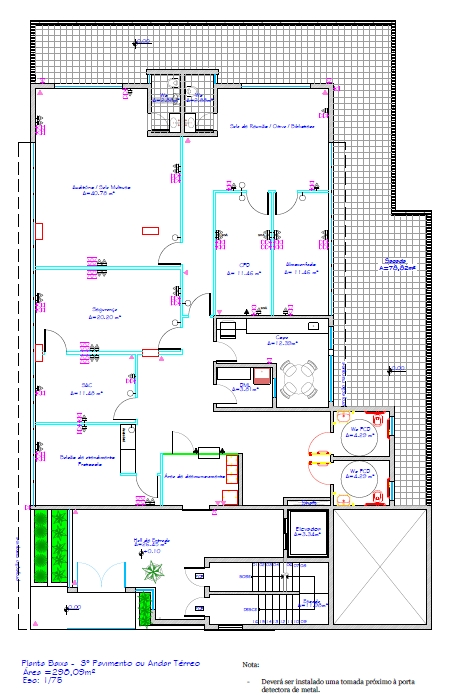
\includegraphics[width=\textwidth]{fig1}
	\caption{Planta baixa térreo}
	\label{fig1}
\end{figure}

\begin{figure}
	\centering
	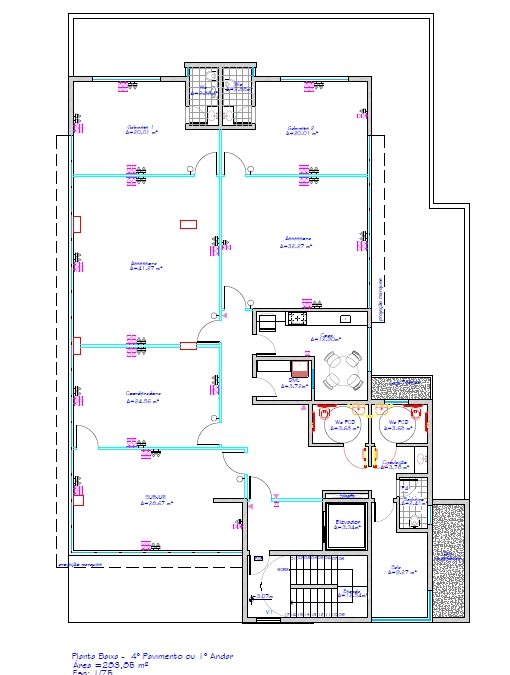
\includegraphics[width=\textwidth]{fig2}
	\caption{Planta baixa andar 1}
	\label{fig2}
\end{figure}

\begin{figure}
	\centering
	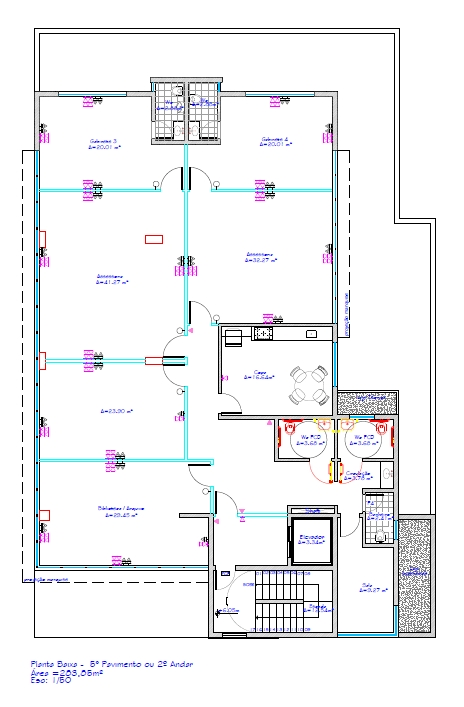
\includegraphics[width=\textwidth]{fig3}
	\caption{Planta baixa andar 2}
	\label{fig3}
\end{figure}

\begin{figure}
	\centering
	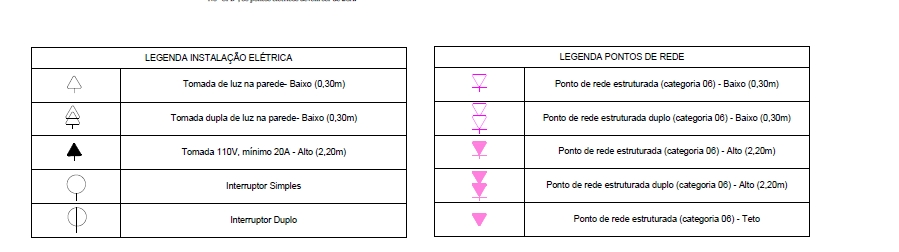
\includegraphics[width=\textwidth]{leg}
	\caption{legenda}
	\label{leg}
\end{figure}

\begin{figure}
	\centering
	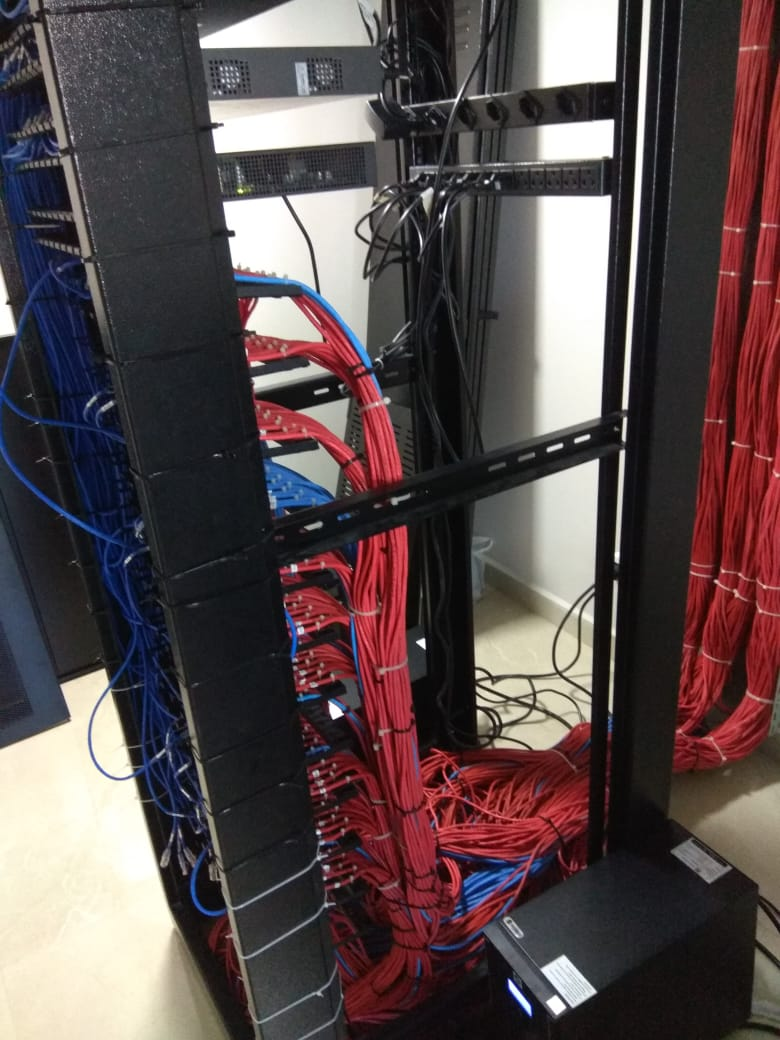
\includegraphics[width=\textwidth]{fig4}
	\caption{cabeamento horizontal concentrado no rack}
	\label{leg}
\end{figure}

\begin{figure}
	\centering
	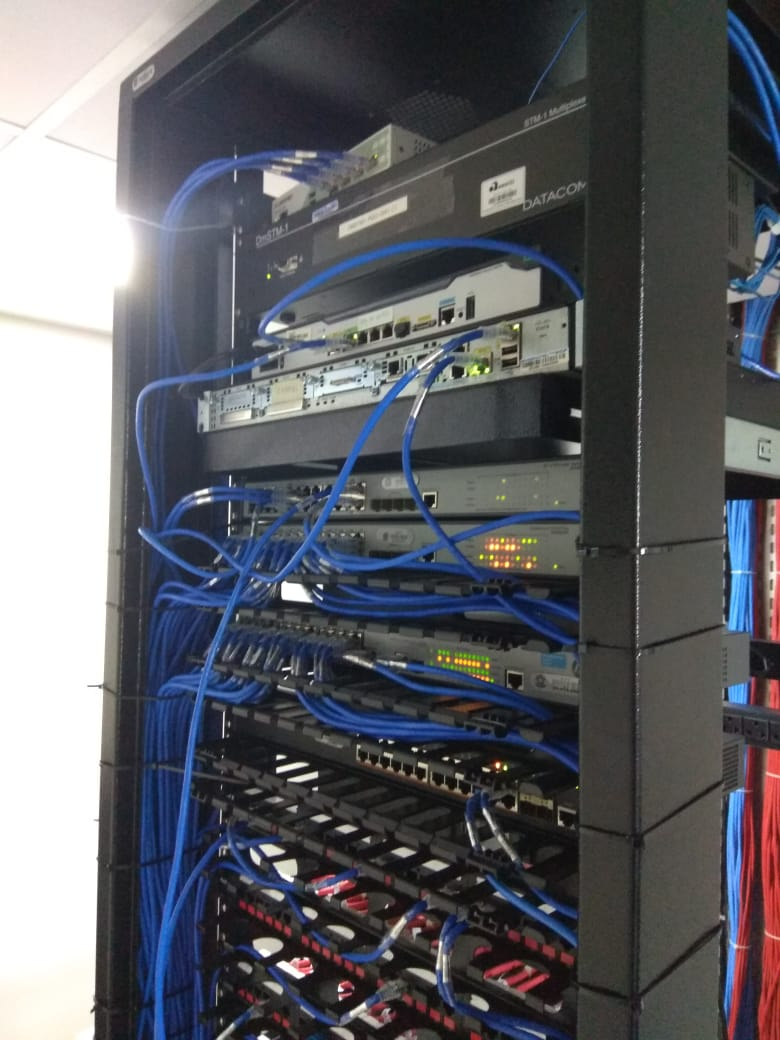
\includegraphics[width=\textwidth]{fig5}
	\caption{swtiches e links de dados}
	\label{leg}
\end{figure}



\subsection{Topologia}

O CPD ficará no térreo, o cabeamento horizontal passará pelos eletrodutos chegando até o patch panel, sendo que a maioria dos pontos terá um cabo e outros passarão 2 cabos. Será utilizado um rack de piso 44U, apenas para os patch panels, swiches e os links de dados e voz, com redundância, como na figura 4. O tamanho do rack já prevê futuras expansões tanto de cabeamento quanto de instalação de servidores e outros equipamentos no rack. A figura 4 traz a concentração do cabeamento horizontal no rack, e a figura 5, temos 4 switches de 26 portas, sendo 2 desses com POE, além do roteador embratel e do enlace de fibra óptica e a redundância. 



\subsection{Encaminhamento}
Os cabos foranm lançados por meio dos eletrodutos já instalados nas paredes que levam diretamente ao CPD no térreo. Os eletrodutos são da marca Tigre e cor amarela e são do tamanho de 3/4". Para maioria dos pontos serão lançado apenas 2 cabos, sendo que os pontos que precisam de impressoras ao lado dos computadores comportarão 3 cabos. Junto às estações de trabalho haverão telefones IP. Os cabos serão lançados por meio de guia para facilitar o lançamento. 

\subsection{Memorial descritivo}

\begin{itemize}

\item 01	Patch Panel 2U 48 portas Fugukawa Gigalan Cat6;
\item 100	Patch Cords 1,5m Furukawa Gigalan Cat6 cor azul;
\item 30	Patch Cords 3m Furukawa Gigalan Cat6 cor azul;
\item 20	Patch Cords 5m Furukawa Gigalan Cat6 cor vermelha;
\item 200	Conectores RJ45 fêmea Fugukawa Gigalan Cat6;
\item 100 	Espelhos 1 posição Furukawa;
\item 50 	Espelhos 2 posição Furukawa;
\item 02	Caixas (305m cada) de cabo de rede UTP Fugukawa Gigalan Cat6 cor vermelha;
\item 01 	Rack fechado de piso 44U IPMETAL (800mm) já com 2 bandejas; guias verticais; 2 guias horizontais e 02 réguas com 12 tomadas 10A;
\item 01	Nobreak de piso 2U 3 KVA NHS 
\end{itemize}

\subsection{Identificação dos cabos}
O cabeamento estruturado serão identificados da seguinte forma. A cada patch panel será atribuída uma letra, nos pontos finais haverá a identificação do andar(01, 02 ou 03), a letra, e por fim a porta do patch panel. Já na ligação aos swiches, optou-se por identificar no patchcord, de maneira não convencional, nas duas pontas, em qual switch e porta aquele cabo está ligado. Essa nomenclatura foi adotada considerando a facilidade para manutenção.

\section{Implantação}
O cronograma de implantação será, respectivamente, a montagem do rack, instalação dos cabos, identificação dos cabos e os testes.
Todo o cabeamento; conectores; wallplates; patch cords e patech panel serão da marca Furukawa Gigalan padrão cat6. O rack e demais acessórios do rack (guias verticais; bandejas fixas; guias de cabo; régua de tomadas) serão da marca IpMetal. Os colaboradores responsáveis pela instalação e montagem optaram pela instalação do padrão EIA/TIA 568A para o cabeamento e terão um cronograma de 8 dias para realizar todo o trabalho. Estes dias serão definidos entre a equipe e o coordenador da unidade.

\section{Plano de certificação}
Ainda que de reconhecida importância para o bom funcionamento a longo prazo da referida rede, o projeto não contará com plano de certificação, considerando os alto custo que envolve a certificação. 

\section{Plano de manutenção}
Não há previsão de expansão de novos pontos, pois a rede já foi projetada com um número de pontos muito além da demanda atual. Contudo, há previsão de aquisição de mais switches uma vez que os que o MPF tem hoje não permitem que todos os pontos à disposição sejam interconectados.

\subsection{Plano de expansão}

Não há previsão de expansão, apenas que sejam adquiridos Access points para o serviço de rede sem fio, tanto para usuários internos quanto para visitantes. A depender de disponibilidade de orçamento.

%%\section{Risco}
%%Enumerar e explicar os riscos do projeto.

%%\section{Orçamento}
%%Crie uma relação de orçamentos baseado na seções anteriores.

%%\section{Recomendações}
%%Observações e recomendações para o cliente.

\section{Referências bibliográficas}
%%Utilize o mendley, o jabref ou diretamente o bibtex para gerenciar suas referências biliográficas. %%As referências são criadas automaticamente de acordo com o uso no texto.
%%Exemplo: Redes de computadores, segundo \cite{t2013} é considerada..... Já \cite{kurose2010} %%apresenta uma versão...
%%Analisando os pressupostos de \cite{ref3} e \cite{ref4} concluimos que....
\renewcommand\refname{} %%Referências bibliográficas}  
\bibliographystyle{ieeetr}
\bibliography{referencias}  

%% ***********************************************************************

\end{document}